\let\negmedspace\undefined
\let\negthickspace\undefined
\documentclass[journal]{IEEEtran}
\usepackage[a5paper, margin=10mm, onecolumn]{geometry}
%\usepackage{lmodern} % Ensure lmodern is loaded for pdflatex
\usepackage{tfrupee} % Include tfrupee package

\setlength{\headheight}{1cm} % Set the height of the header box
\setlength{\headsep}{0mm}     % Set the distance between the header box and the top of the text

\usepackage{gvv-book}
\usepackage{gvv}
\usepackage{cite}
\usepackage{amsmath,amssymb,amsfonts,amsthm}
\usepackage{algorithmic}
\usepackage{graphicx}
\usepackage{textcomp}
\usepackage{xcolor}
\usepackage{txfonts}
\usepackage{listings}
\usepackage{enumitem}
\usepackage{mathtools}
\usepackage{gensymb}
\usepackage{comment}
\usepackage[breaklinks=true]{hyperref}
\usepackage{tkz-euclide} 
\usepackage{listings}
% \usepackage{gvv}                                        
\def\inputGnumericTable{}                                 
\usepackage[latin1]{inputenc}                                
\usepackage{color}                                            
\usepackage{array}                                            
\usepackage{longtable}                                       
\usepackage{calc}                                             
\usepackage{multirow}                                         
\usepackage{hhline}                                           
\usepackage{ifthen}
\usepackage{lscape}
\begin{document}

\bibliographystyle{IEEEtran}

\title{10.7.105}
\author{EE25BTECH11057 - Rushil Shanmukha Srinivas
}
% \maketitle
% \newpage
% \bigskip
{\let\newpage\relax\maketitle}

\renewcommand{\thefigure}{\theenumi}
\renewcommand{\thetable}{\theenumi}
\setlength{\intextsep}{10pt} % Space between text and floats

\numberwithin{equation}{enumi}
\numberwithin{figure}{enumi}
\renewcommand{\thetable}{\theenumi}
\textbf{Question: }
Consider the parabola $y^2 = 4x$. Let $\vec{S}$ be the focus of the parabola. A pair of tangents
drawn to the parabola from the point $\vec{R}$ = (-2,1) meet the parabola at $\vec{R_1}$ and $\vec{R_2}$ .
Let $\vec{Q_1}$ and $\vec{Q_2}$ be points on the lines $S{R_1}$ and $S{R_2}$ respectively such that $RQ_1$ is
perpendicular to $SR_1$ and $RQ_2$ is perpendicular to $SR_2$ . Then, which of the following
is/are TRUE ?
\begin{multicols}{2}
\begin{enumerate}
\item $SQ_1$ = 2
\item $Q_1Q_2$ = $\frac{3\sqrt{10}}{5}$
\item $RQ_1$ = 3
\item $SQ_2$ = 1
\end{enumerate}
\end{multicols}
\textbf{Solution: }
\begin{table}[h!]
  \centering
  \begin{tabular}{|c|c|}
\hline
\textbf{Name} & \textbf{Value} \\
\hline
Parabola & $\vec{x}^\top\myvec{0&0\\0&1}\vec{x} - \myvec{4 & 0}\vec{x} = 0$ \\
\hline
\end{tabular}

  \caption*{Table : Conics}
  \label{10.7.105}
\end{table}

On comparing Parabola  with
\begin{align}
\vec{x}^\top\vec{V}\vec{x} + 2\vec{u}^\top\vec{x} + f &= 0 \label{eq: conic}
\end{align}
The parameters of the Parabola are 
\begin{align}
\vec{V}=\myvec{0&0\\0&1} , \vec{u}=\myvec{-2\\0} , f=0
\end{align}
As $\vec{V}$ is an upper triangular matrix , we get the eigen values as the diagonal entries 
\begin{align}
  \lambda_1 &= 0 & \lambda_2 = 1
\end{align}
For a Symmetric Matrix, we have the Eigen decomposition
\begin{align}
\vec{V} = \vec{P}\vec{D}\vec{P}^\top
\end{align}
\begin{align}
\vec{D} = \myvec{\lambda_1&0\\0&\lambda_2} = \myvec{0&0\\0&1} = \vec{V}
\end{align}
\begin{align}
\vec{P} = \myvec{\vec{p_1}&\vec{p_2}} \ and \ \vec{P}^\top\vec{P} = \vec{I} 
\end{align}
Solving both 
\begin{align}
\vec{V} = \vec{P}\vec{V}\vec{P}^\top \ and \ \vec{P}^\top\vec{P} = \vec{I}
\end{align}
We get
\begin{align}
\vec{P} = \myvec{\pm1&0\\0&\pm1}
\end{align}
So
\begin{align}
\vec{p_1} = \myvec{\pm1\\0} \ and \ \vec{p_2} = \myvec{0\\ \pm1}
\end{align}
For a parabola, Eccentricity = e = 1
\begin{align}
\vec{n} = \sqrt{\lambda_2}\vec{p_1} = \vec{p_1} = \myvec{1\\0}
\end{align}
\begin{align}
c = \frac{{\norm{\vec{u}}}^2 - \lambda_2 f}{2\vec{u}^\top\vec{n}} = \frac{4}{-4} = -1
\end{align}
\begin{align}
Focus = \vec{F} = \vec{S} = \frac{ce^2\vec{n} - \vec{u}}{\lambda_2} = \myvec{1\\0}
\end{align}
Given,
\begin{align}
\vec{R} = \myvec{-2\\1}
\end{align}
Given, The point of contact $\vec{q}$ the equation of tangent to \eqref{eq: conic} is
\begin{align}
\brak{\vec{V}\vec{q}+\vec{u}}^\top\vec{x} + \vec{u}^\top\vec{q} + f = 0
\end{align}
As the tangent passes through $\vec{R}$
\begin{align}
\brak{\vec{V}\vec{q}+\vec{u}}^\top\vec{R} + \vec{u}^\top\vec{q} + f = 0
\end{align}
Also $\vec{q}$ lies on the conic
\begin{align}
\vec{q}^\top\vec{V}\vec{q} + 2\vec{u}^\top\vec{q} = 0 \label{eq: 0}
\end{align}
\begin{align}
\vec{V}^\top = \vec{V} , \brak{\vec{V}\vec{q}+\vec{u}}^\top\vec{R} + \vec{u}^\top\vec{q} = \vec{q}^\top\vec{V}\vec{R} + \vec{u}^\top\vec{R} + \vec{u}^\top\vec{q} = 0 \label{eq: 1}
\end{align}
\begin{align}
\vec{V}\vec{R} = \myvec{0\\1} \ and \ \vec{V}\vec{R} + \vec{u} = \vec{R} \ and \ \vec{u}^\top\vec{R} = 4
\end{align}
Also
$
\vec{q}^\top\vec{V}\vec{R} , \vec{R}^\top\vec{V}\vec{q} \ are \ scalars.
$
For a scalar the transpose of a scalar is the same scalar.So
\begin{align}
\vec{q}^\top\vec{V}\vec{R} = \brak{\vec{q}^\top\vec{V}\vec{R}}^\top = \vec{R}^\top\vec{V}\vec{q}
\end{align}
From \eqref{eq: 1}
\begin{align}
\vec{q}^\top\vec{V}\vec{R} + 4 + \brak{\vec{R}-\vec{V}\vec{R}}^\top\vec{q} = 0 \\
\vec{q}^\top\vec{V}\vec{R} + 4 + \vec{R}^\top\vec{q} - \vec{R}^\top\vec{V}\vec{q} = 0 \\
\vec{R}^\top\vec{q} = -4
\end{align}
$\vec{q}$ can be expressed as combination of $\vec{R}$ and its orthogonal component
\begin{align}
\vec{q} = \lambda\vec{R} + \vec{z} , \ where \ \vec{R}^\top\vec{z} = 0 \label{eq: 2}
\end{align}
\begin{align}
\vec{R}^\top\vec{q} = \lambda\vec{R}^\top\vec{R} = -4 \\
\lambda = \frac{-4}{5}
\end{align}
Substituting \eqref{eq: 2} in \eqref{eq: 0}
\begin{align}
\lambda^2\vec{R}^\top\vec{V}\vec{R} + 2\lambda\vec{R}^\top\vec{V}\vec{z} + \vec{z}^\top\vec{V}\vec{z} + 8\lambda + 2\vec{u}^\top\vec{z} = 0
\end{align}
\begin{align}
\vec{R}^\top\vec{V}\vec{R} = 1 \ and \ \lambda = \frac{-4}{5}
\end{align}
Substituting these and simplifying the equation
\begin{align}
25\vec{z}^\top\vec{V}\vec{z} - 40\vec{R}^\top\vec{V}\vec{z} + 50\vec{u}^\top\vec{z} - 144 = 0 \label{eq: 3}
\end{align}
\begin{align}
\vec{z} = \myvec{\frac{-\vec{u}^\top\vec{z}}{2}\\\vec{R}^\top\vec{V}\vec{z}}
\end{align}
\begin{align}
\vec{R}^\top\vec{z} = 0 \Longrightarrow \vec{R}^\top\vec{V}\vec{z} = -\vec{u}^\top\vec{z} 
\end{align}
Let
\begin{align}
\vec{R}^\top\vec{V}\vec{z} = -\vec{u}^\top\vec{z} = k
\end{align}
Then
\begin{align}
\vec{z}^\top\vec{V}\vec{z} = \brak{\vec{R}^\top\vec{V}\vec{z}}^2 = k^2
\end{align}
Then from \eqref{eq: 3}
\begin{align}
25k^2 - 90k - 144 = 0 \\
\brak{k - \frac{24}{5}}\brak{k + \frac{6}{5}} = 0 \\
k = \frac{24}{5} \ or \ k=\frac{-6}{5} \\
\vec{z} = \frac{1}{5}\myvec{12\\24} \ or \ \vec{z} = \frac{1}{5}\myvec{-3\\-6} \\
\vec{q} = \myvec{4\\4} \ or \ \vec{q} = \myvec{1\\-2}
\end{align}
As $\vec{R_1}$,$\vec{R_2}$ are the point of contact of Tangents $\{\vec{R_1},\vec{R_2}\}$ $\in$ $\vec{q}$
\begin{align}
\vec{R_1} = \myvec{4\\4} \ and \ \vec{R_2} = \myvec{1\\-2}
\end{align}
If $\vec{A}$,$\vec{B}$ are on line $\vec{h}^\top\vec{x}=d$ then
\begin{align}
\myvec{\vec{A} & \vec{B}}^\top\vec{h} = \myvec{1\\1}
\end{align}
For the line passing through $\vec{R_1}$ and $\vec{S}$
\begin{align}
\myvec{4&4\\1&0}\vec{h} = \myvec{1\\1}
\end{align}
The augmented Matrix is
\begin{align}
  \myaugvec{2}{4 & 4 & 1\\1 & 0 & 1} \xleftrightarrow{R_2 \longrightarrow R_2-\frac{R_1}{4}} 
  \myaugvec{2}{4 & 4 & 1\\0 & -1 & \frac{3}{4}} \xleftrightarrow{R_1 \longrightarrow R_1+4R_2}
\myaugvec{2}{4 & 0 & 4\\0 & -1 & \frac{3}{4}} \\
\myaugvec{2}{4 & 0 & 4\\0 & -1 & \frac{3}{4}} \xleftrightarrow{R_1 \longrightarrow \frac{-R_1}{4}} \myaugvec{2}{-1 & 0 & -1\\0 & -1 & \frac{3}{4}}
\end{align}
\begin{align}
\vec{h} = \myvec{1\\ \frac{-3}{4}} = \frac{1}{4}\myvec{4\\-3} , \vec{m} = \myvec{3\\4}
\end{align}
The equation of the line through $\vec{R_1},\vec{S}$ is
\begin{align}
\myvec{4&-3}\vec{x} = 4  \label{eq: line1}
\end{align}
For the line passing through $\vec{R_2}$ and $\vec{S}$
\begin{align}
\myvec{1&-2\\1&0}\vec{h} = \myvec{1\\1}
\end{align}
The augmented Matrix is
\begin{align}
  \myaugvec{2}{1 & -2 & 1\\1 & 0 & 1} \xleftrightarrow{R_2 \longrightarrow R_2-R_1} 
  \myaugvec{2}{1 & -2 & 1\\0 & 2 & 0} \xleftrightarrow{R_1 \longrightarrow R_1+R_2}
\myaugvec{2}{1 & 0 & 1\\0 & 2 & 0} \\
\myaugvec{2}{1 & 0 & 1\\0 & 2 & 0} \xleftrightarrow{R_2 \longrightarrow \frac{R_2}{2}} \myaugvec{2}{1 & 0 & 1\\0 & 1 & 0}
\end{align}
\begin{align}
\vec{h} = \myvec{1\\ 0}  , \vec{m} = \myvec{0\\2}
\end{align}
The equation of the line through $\vec{R_2},\vec{S}$ is
\begin{align}
\myvec{1&0}\vec{x} = 1   \label{eq: line2}
\end{align}
If $\vec{Q}$ be the foot of perpendicular from $\vec{T}$ to the line $\vec{h}^\top\vec{x} = d$ then
\begin{align}
\myvec{\vec{m}&\vec{h}}^\top\vec{Q} = \myvec{\vec{m}^\top\vec{T}\\d}
\end{align}
$\vec{Q_1}$,$\vec{Q_2}$ are foot of perpendicular drawn from $\vec{R}$ to \eqref{eq: line1} and \eqref{eq: line2}.
So
\begin{align}
\myvec{3&4\\4&-3}\vec{Q_1} = \myvec{-2\\4} \label{eq: relation1}
\end{align}
\begin{align}
\myvec{0&2\\1&0}\vec{Q_2} = \myvec{2\\1}  \label{eq: relation2}
\end{align}
The augmented Matrix for \eqref{eq: relation1} is
\begin{align}
  \myaugvec{2}{3 & 4 & -2\\4 & -3 & 4} \xleftrightarrow{R_2 \longrightarrow 3R_2-4R_1} 
  \myaugvec{2}{3 & 4 & -2\\0 & -25 & 20} \xleftrightarrow{R_1 \longrightarrow 25R_1+4R_2}
\myaugvec{2}{75 & 0 & 30\\0 & -25 & 20} \\
\myaugvec{2}{75 & 0 & 30\\0 & -25 & 20} \xleftrightarrow{R_2 \longrightarrow \frac{-R_2}{25}} \myaugvec{2}{75 & 0 & 30\\0 & 1 & \frac{-4}{5}} \xleftrightarrow{R_1 \longrightarrow \frac{R_1}{75}} \myaugvec{2}{1 & 0 & \frac{2}{5}\\0 & 1 & \frac{-4}{5}}
\end{align}
\begin{align}
\vec{Q_1} = \myvec{\frac{2}{5}\\ \frac{-4}{5}} = \frac{1}{5}\myvec{2\\-4}
\end{align}
The augmented Matrix for \eqref{eq: relation2} is
\begin{align}
  \myaugvec{2}{0 & 2 & 2\\1 & 0 & 1} \xleftrightarrow{R_1 \longrightarrow \frac{R_1}{2}} 
  \myaugvec{2}{0 & 1 & 1\\1 & 0 & 1} \xleftrightarrow{R_1 \longleftrightarrow R_2}
\myaugvec{2}{1 & 0 & 1\\0 & 1 & 1} 
\end{align}
\begin{align}
\vec{Q_2} = \myvec{1\\ 1} 
\end{align}
\begin{align}
SQ_1 = \norm{\vec{S}-\vec{Q_1}} = \norm{\frac{1}{5}\myvec{3\\4}} = 1 \\
Q_1Q_2 = \norm{\vec{Q_1}-\vec{Q_2}} = \norm{\frac{1}{5}\myvec{3\\9}} = \frac{3\sqrt{10}}{5} \\
RQ_1 = \norm{\vec{R}-\vec{Q_1}} = \norm{\frac{1}{5}\myvec{-12\\9}} = 3 \\
SQ_2 = \norm{\vec{S}-\vec{Q_2}} = \norm{\myvec{0\\-1}} = 1
\end{align}
So options 2,3,4 are correct.
\begin{figure}[h!]
  \centering
  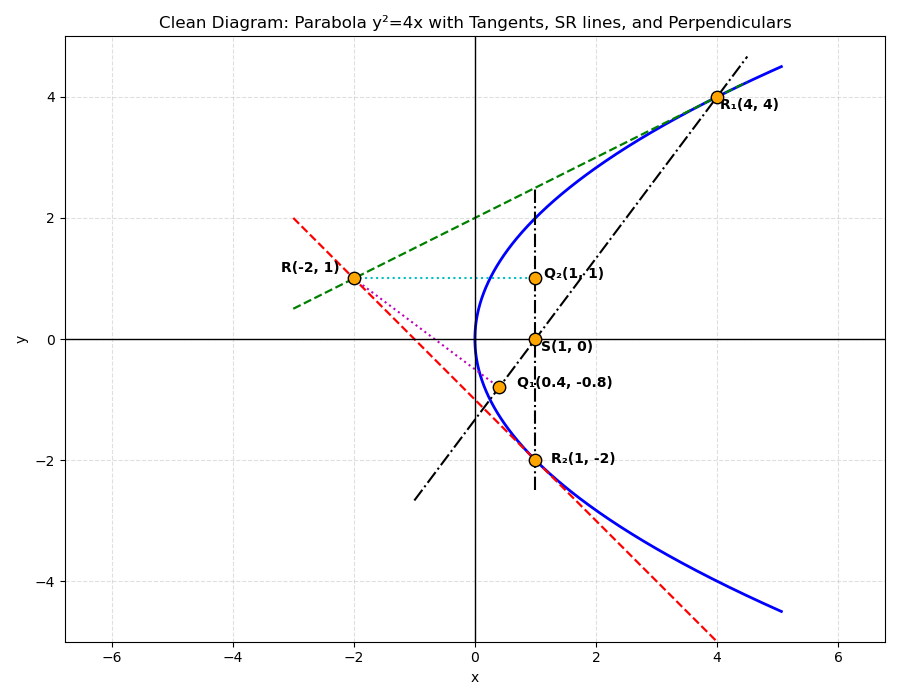
\includegraphics[width=0.9\columnwidth]{figs/fig18.png} 
   \caption*{Fig : Parabola and Tangents }
  \label{Fig1}
\end{figure}

\end{document}